%*****************************************
\chapter{Stand der Forschung}\label{ch:relatedWork}
%*****************************************

\section{Health IT Ontology}

\subsection{Allgemein}

Die Welt der medizinischen Informatik umfasst eine Vielzahl an Begriffen, Werkzeugen und Prozessen. 
Dies führt beim Vergleich von IT-Komponenten im Gesundheitswesen, aufgrund von diversen Terminologien zu Schwierigkeiten. 
Aus diesem Grund wurde \ac{HITO} ins Leben gerufen.
\ac{HITO} ermöglicht eine systematische Beschreibung von Anwendungssystemen und Softwareprodukten innerhalb von Krankenhausinformationssystemen.
So unterstützt \ac{HITO} das Management, die Weiterbildung und die Lehre im Bereich der medizinischen Informatik.

\subsection{Use Cases}\label{sec:usecases}

Use Cases beschreiben Situationen in denen ein Produkt genutzt werden kann.
Im folgenden werden die Use Cases für HITO aus dem Projektantrag \citep{winter_haux} erläutert. \newline

\textbf{Use Case 1}: Mitarbeiter des Informationsmanagements möchten in einer \ac{KIS} Strategiebesprechung, die existierenden Komponente des \ac{KIS} für alle Teilnehmer verständlich erklären.
Im Idealfall verfügen alle Teilnehmer über die selbe Terminologie.
Das ist aber in der Realität anders, da die Teilnehmer aufgrund der individuellen Spezialisierungen und Fachbereiche jeweils unterschiedliche Terminologien verwenden. \newline

\textbf{Use Case 2}:  Mitarbeiter des Informationsmanagements möchten ein neues Softwareprodukt für das Krankenhausinformationssystem auswählen.
In dieser Situation entstehen Fragen wie zum Beispiel: \enquote{Wie wählt man Software-Produkte für das \ac{KIS} von dem Markt aus?} oder \enquote{Welche andere Organisationen haben ähnliche Anwendungssysteme im Rahmen ihres \ac{KIS}}
In diesem Fall steht man vor der Herausforderung, dass Software-Hersteller unterschiedliche Terminologien für die Beschreibung ihrer Software-Produkte nutzen.
Somit lassen sich diese Beschreibungen nicht vergleichen. \newline

\textbf{Use Case 3}: Mitarbeiter des Informationsmanagements, die über geringe finanzielle Ressourcen verfügen, möchten ein Anwendungssystem installieren, das ein \ac{LIFOSS} Produkt ist.
In diesem Fall, möchten sich Mitarbeiter über die verfügbaren \ac{LIFOSS} Produkte und deren Eigenschaften informieren.
Das Problem bei diesem Use-Case besteht darin, dass \ac{LIFOSS} Produkte nicht so gut vermarktet sind wie kommerzielle Software-Produkte. 
In diesem Fall stolpert(besseres Wort finden) man zusätzlich auch, über die im Use Case 2 beschriebene Herausforderung. \newline

\textbf{Use Case 4}: Mitarbeiter des Informationsmanagements möchten sich bezüglich eines KIS-Anwendungssystems oder eines Software-Produkts evidenzbasierte Daten anschauen.  \newline

\textbf{Use Case 5}: Mitarbeiter des Informationsmanagements möchten neue Mitarbeiter einstellen oder das existierende Personal weiterbilden.
Dafür muss eine Liste an Anforderungen zusammengestellt werden.
In diesem Fall kommen Fragen wie zum Beispiel: \enquote{Welche Ausbildungen werden für bestimmte Software Produkte angeboten?} oder \enquote{Welche Spezialisten mit bestimmte Kompetenzen sind aktuell auf dem Arbeitsmarkt verfügbar?}.
Hier besteht das Problem, dass diese Art von Informationen nicht systematisch aufbereitet sind, sondern nur als Freitext verfügbar sind.\newline

\subsection{Aufbau}

Der Aufbau der Ontologie wird in der Abbildung \ref{fig:metamodel} dargestellt. 
In den Klassen enthaltenen Instanzen bilden die Wissensbasis.
Zum Beispiel enthält die zentrale Klasse \enquote{SoftwareProduct} 52 Instanzen.
Die Tabelle \ref{tab:hito_klassen} enthält alle Klassen von HITO mit einer Beschreibung.

\begin{sidewaysfigure}[ht]
    	\includegraphics[width=\textwidth]{Images/hito_metamodell}
   	\caption{HITO -- Ontologie}
	\caption*{\small Quelle: \url{https://hitontology.eu/public/2022-05-hito_diagram.svg}}
   	\label{fig:metamodel}
\end{sidewaysfigure}

\clearpage

\begin{longtable}[ht]{p{3,5cm} p{8cm}}
\toprule
Klasse									&Definition\\
\midrule
\endhead
Application System Type Catalogue & Eine Sammlung von klassifizierten Anwendungssystemen. \\
Application System Type Citation & Der Begriff, den ein Autor für das Anwendungssystem verwendet, das in der Studie bewertet wird. \\
Application System Type Classified & Der Begriff für ein Anwendungssystem, der in der Klassifizierung von Anwendungssystemen verwendet wird. \\
Catalogue & Eine Sammlung von klassifizierten Begriffe der gleichen Art aus der gleichen Quelle. \\
Certification & Zertifikat eines Softwareprodukts zur Bewertung der Einhaltung der Normen des Qualitätsmanagements. \\
Citation & Beschreibung eines Softwareprodukts in natürlicher Sprache anhand der Produktdokumentation, z. B. einer Webseite. \\
Classified & Klassifiziert einen Eintrag eines Katalogs, wie z.B. ein Merkmal oder eine Unternehmensfunktion. \\
Client & Die Art der Hardware- und Softwareumgebung, auf der ein Softwareprodukt ausgeführt werden kann. \\
Database System & Database Management System, wie z.B. MySQL oder PostgreSQL.\\
Enterprise Function Citation & Das natürlichsprachliche Zitat einer Unternehmensfunktion beschreibt, was die handelnden Menschen oder Maschinen in einem bestimmten Unternehmen zu tun haben, um zu dessen Aufgabe oder Zielen beizutragen. Eine Unternehmensfunktion ist eine Richtlinie in einer Institution, wie Daten über Entitätstypen zu interpretieren sind und dann Daten über Entitätstypen als Folge dieser Interpretation zu aktualisieren sind. Das Zitat ist ein Begriff, den ein Autor verwendet, um die Unternehmensfunktion zu beschreiben, die durch ein Anwendungssystem unterstützt wird. \\
Enterprise Function Classified & Der Begriff für eine Unternehmensfunktion, der in der Klassifizierung von Unternehmensfunktionen verwendet wird. Es ist ein klassifizierter Begriff im Sinne unserer Definition, der zu einer Klassifikation gehört. \\
Experimental Study RCT &  Experimentelle Studie mit randomisiertem Kontrollversuch. \\
Feature Catalogue & Eine Sammlung von klassifizierten Softwarefunktionen. \\
Feature Citation & Features sind vom Softwareprodukt des Anwendungssystems angebotene Funktionalitäten, die direkt zur Erfüllung einer oder mehrerer Funktionen beitragen. Je feiner die Granularität einer Funktion formuliert ist, desto größer ist die Wahrscheinlichkeit, dass die Funktion semantisch mit einem Feature einer Anwendungskomponente übereinstimmt. \\
Feature Classified & Der zusammenfassende Begriff eines Merkmals, der in Katalogen verwendet wird. Es ist ein klassifizierter Begriff nach unserer Definition, der zu einer Klassifikation gehört.  \\
Function Catalogue & Eine Sammlung von klassifizierten Unternehmensfunktionen. \\
Interoperability & Interoperabilität ist im Allgemeinen die Fähigkeit von zwei oder mehr Komponenten, Informationen auszutauschen und die ausgetauschten Informationen zu nutzen. Normen bieten eine gemeinsame Sprache und eine Reihe gemeinsamer Erwartungen, die die Interoperabilität zwischen Systemen und/oder Geräten ermöglichen. Um Informationen über eine Person nahtlos zu verarbeiten und die Gesamtkoordination und -bereitstellung der Gesundheitsversorgung zu verbessern, ermöglichen Normen Ärzten, Labors, Krankenhäusern, Apotheken und Patienten den Austausch von Daten unabhängig von der Anwendung oder dem Marktanbieter. \\
Journal & Wissenschaftliche Zeitschrift. \\
Lab Study & Laborstudie. \\
Language & Sprache. \\
Non Experimental Study & Nicht-experimentelle Studie. \\
Operating System & Die DBpedia-Instanzen wurden unter dieser HITO-Klasse gebündelt, da DBpedia nicht gut geeignet war. \\
Organizational Unit Catalogue & Eine Sammlung von klassifizierten Organisationseinheiten. \\
Organizational Unit Citation & Der Begriff, den ein Autor für die Organisationseinheit verwendet, in der die Auswertung des Anwendungssystems stattfindet. \\
Organizational Unit Classified & Klassifizierter Katalogeintrag einer Organisationseinheit. Das SNOMED CT-Konzept von SNOMED International. \\
Outcome Criteria \newline Citation & Der Begriff, den ein Autor für die Ergebniskriterien der Bewertungsstudie verwendet. \\
Outcome Criteria Classified & Klassifizierter Katalogeintrag eines Ergebniskriteriums. \\
PMID & The PMID extracted from PubMed for each study. \\
Programming \newline Language & Programmiersprache. \\ 
Programming \newline Library & Eine Programmierbibliothek ist eine Sammlung von wiederverwendbarem Code. \\
Quasi Experimental Study & Empirische Interventionsstudie ohne Randomisierung. \\
Software Product & Ein Softwareprodukt ist ein erworbenes oder selbst entwickeltes Softwareprgramm, das auf einem Computersystem installiert werden kann. \\
Software Product \newline Installation & Also known as Computer-based application component. Based on a software product, which is an acquired or self-developed piece of software that can be installed on a computer system. For example, the computer-based application component patient administration system stands for the installation of a software product to support enterprise functions such as patient admission and administrative discharge and final billing. \\
Study & Eine Evaluationsstudie. \\
Study Method \newline Citation & The natural language term an author uses for a study method which is used in the evaluation study. \\
Study Method \newline Classified & The study method, qualitative or quantitative. \\
User Group \newline Catalogue & A collection of classified user groups. \\
User Group Citation & Der Begriff, den ein Autor für die Benutzergruppe eines Anwendungssystems verwendet. \\
User Group \newline Classified & Das SNOMED CT-Konzept von SNOMED International. SNOMED CT - Internationaler SNOMED CT Browser [Internet]. Release: International Edition 20190131. 2019 [cited 2019 Mar 26]. Verfügbar unter: https://browser.ihtsdotools.org/? \\
Validation Study & Vergleicht die Genauigkeit einer Messung mit einer Standardmessung.\\
\bottomrule
\caption[Klassen der Ontologie]{Klassen der Ontologie \newline \small Quelle: \url{https://hitontology.github.io/ontology/}}
\label{tab:hito_klassen}
\end{longtable}

\section{Human-Computer Interaction}\label{sec:ux}

Die Art und Weise in der Menschen mit Computer interagieren hat sich über die Jahre stark verändert und steht in einer kontinuierlichen Entwicklung. 
Der Begriff  \ac{HCI}, zu Deutsch \ac{MMI} oder \ac{MCI}, wurde in den 1980er eingeführt.
Mit diesem Begriff wurde bestätigt, dass der Fokus nicht nur auf das Design der Benutzeroberfläche liegt, sondern alle Aspekte, die die Interaktion zwischen Nutzer und Computern betreffen, zu beachten sind. \citep[vgl.]{preece_human-computer_1995}
Ziel der Forschung im Rahmen von \ac{HCI} ist die stetige Verbesserung der Interaktion zwischen Menschen und Computern. \newline

\noindent Im Laufe der Jahre hat sich keine einheitliche Definition für \ac{HCI} etabliert.
Die \enquote{Encyclopedia of Database Systems} von \citet{dix_human-computer_2009} definiert \ac{HCI} wie folgt:
\begin{definition}
  \enquote{Human–Computer Interaction (HCI) is the study of the way in which computer technology influences human work and activities. 
  The term ‘‘computer technology’’ now-a-days includes most technology from obvious computers with screens and keyboards to mobile phones, household appliances, in-car navigation
  systems and even embedded sensors and actuators such as automatic lighting. 
  HCI has an associated design discipline, sometimes called Interaction Design or UserCentered Design, focused on how to design computer technology so that it is as easy and
  pleasant to use as possible.}
\end{definition}

\noindent Im Vergleich dazu definiert \citet{heimgartner_interkulturelles_2017}  \ac{HCI}  wie folgt:

\begin{definition}
  \enquote{Die Interaktion, bei der Information zwischen Benutzer und System via Benutzungsschnittstelle \ac{UI}) ausgetauscht wird, wird als \enquote{\ac{MMI}}  oder  \enquote{\ac{MCI}} bezeichnet.}
\end{definition}

\subsection{User Experience}

 \ac{UX} ist ein weitgreifender Ansatz, der \enquote{alle Aspekte der Erfahrungen eines Nutzers bei der Interaktion mit einem Produkt, Dienst, einer Umgebung oder Einrichtung} umfasst.
Ins Deutsche lässt sich der Begriff am besten als Nutzungserlebnis oder Nutzungserfahrung übersetzen. \citep[vgl.]{jacobsen_praxisbuch_2019}
Die Abbildung \ref{fig:abb2} zeigt, welche Aspekte die \ac{UX} vor, während und nach der Nutzung einer Anwendung betrachtet.
Demnach ist die Usability ein Teil der \ac{UX}.
Im folgenden Unterkapitel wird erläutert, was Usability ist und was man beachten muss, um eine gute Usability zu erreichen.

\begin{figure}[h]
	\centering
    	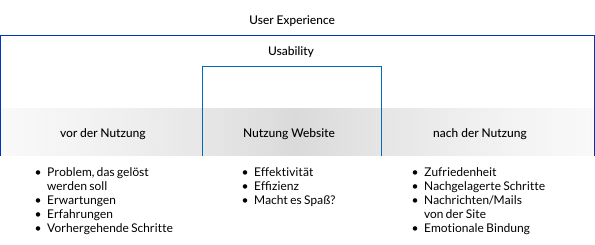
\includegraphics[width=0.99\textwidth]{Images/User_Experience.png}
   	\caption{User Experience}
	\caption*{\small Quelle: \cite{jacobsen_praxisbuch_2019}}
   	\label{fig:abb2}
\end{figure}

Eine gute \ac{UX} zeichnet sich dadurch aus, dass die Nutzer*innen bei der Interaktion positive Emotionen wie zum Beispiel Vorfreude, Spaß oder Zufriedenheit empfinden.
Zudem sollen die Erwartungen der Nutzer*innen erfüllt oder sogar übertroffen werden.
Weitere Faktoren, die die \ac{UX} positiv beeinflussen, sind die Utility, die Ästhetik und die Markenwahrnehmung. \citep[vgl.]{weichert_quick_2021}

\subsection{Usability}

Die ISO-Norm 9241-11 \citep{ISO_standard} bezeichnet Usability als \enquote{das Ausmaß, in dem ein Produkt, System oder Dienst durch bestimmte Benutzer in einem bestimmten Anwendungskontext genutzt werden kann, um bestimmte Ziele effektiv, effizient und zufriedenstellend zu erreichen}.

Daher besteht die Kernfrage der Usability daraus, ob der Nutzer seine Aufgaben und Ziele erfolgreich erreichen konnte.
Aus diesem Grund ist das Ziel von Usability, eine Anwendung so einfach wie möglich für den Benutzer zu gestalten. \citep[vgl.]{jacobsen_praxisbuch_2019}

Folgende Eigenschaften sollen laut der ISO-Norm 9241 \citep{ISO_standard} erfüllt werden, um eine gute Usability zu gewährleisten:

\begin{itemize}
	\item \textbf{Der Aufgabe angemessen:} Die Anwendung soll die Erwartungen der Nutzer erfüllen. Nutzer sollen in der Lage sein ihre Ziele schnell zu erreichen.
	\item \textbf{Selbstbeschreibend:} Dem Nutzer soll ersichtlich sein, wie er sein Ziel erreicht. Die Navigation soll klar und verständlich gestaltet sein.
	\item \textbf{Steuerbar:} In diesem Fall, soll der Benutzer die Anwendung steuern und nicht umgekehrt. Zum Beispiel soll der Nutzer in der Lage sein zur vorherigen Seiten zurück zu springen.
	\item \textbf{Erwartungskonform:} Die Anwendung soll so gestaltet werden, dass Nutzer nicht überrascht werden. Etablierte Verhalten oder Elemente der Benutzeroberfläche sollen berücksichtigt werde. Zudem soll auch die Konsistenz innerhalb der Anwendung beachtet werden.
	\item \textbf{Fehlertolerant:} Falsche Benutzereingaben sollen betrachtet werden. Dabei muss dem Nutzer der Fehler signalisiert werden und eine schnelle Korrektur soll gewährleistet werden.
	\item \textbf{Individualisierbar:} Die Anwendung soll dem Nutzer die Möglichkeit geben, seine Angaben zu speichern und diese bei dem nächsten Besuch nicht erneut eingeben zu müssen.
	\item \textbf{Lernförderlich:} Die Anwendung soll den Benutzer dabei unterstützen, den Umgang schrittweise zu erlernen, beispielsweise durch Tastaturkürzel.
\end{itemize}

\subsection{User-Centered Design}

Das \ac{UCD} ist eine Methodik, die von Software-Entwickler und Designer im Bereich vom Software Design angewendet wird. 
Die Methode hilft dabei Software zu entwickeln, die der Bedürfnisse der Nutzer entspricht. \citep[vgl.]{salinas_2020}

\begin{definition}

\enquote{User-Centered Design bezeichnet ein Vorgehen, das durch die direkte Einbeziehung der Nutzer, frühe Visualisierung in From von Prototypen und ein iteratives Vorgehen sicherstellt, dass die Erwartungen der Nutzer erfüllt oder übertroffen werden und das Nutzungserlebnis positiv ausfällt.} \citep{weichert_quick_2021}

\end{definition} 

Laut dem ISO 13407 Standard, besteht die Methodik aus den vier folgenden Schritte:

\begin{enumerate}
	\item Verstehen und Spezifizieren des Nutzungskontextes (Analyse)
	\item Spezifizierung der Benutzer- und Organisationsanforderungen (Konzeption)
	\item Entwurfslösungen erstellen (Design)
	\item Entwürfe anhand der Anforderungen zu bewerten (Evaluation)
\end{enumerate}



